\documentclass[a4paper,12pt]{article}

\usepackage{graphicx} % Required for inserting images
\usepackage{amsmath,amssymb,amsfonts}
\usepackage{subcaption}
% Use Times New Roman font
\usepackage{times}
\usepackage[a4paper, top=1in, bottom=0.8in, left=1.1in, right=0.8in]{geometry}
\usepackage{float}
\usepackage{listings}
\usepackage{xcolor} % For customizing code colors
\setlength{\parindent}{0pt}
\usepackage{titlesec} % Add this to your preamble
\titleformat{\section}
{\normalfont\large\bfseries}{\thesection}{1em}{}
% Set spacing for sections
\titlespacing*{\section}
{0pt}  % Left spacing
{1ex} % Space before (adjust this value)
{1ex}  % Space after (adjust this value)
\begin{document}
	\section{Experiment No. 3}
	
	
	\section{Experiment Title }
	Design and Analyze a 2 Input NAND and AND Gate Using 1 Finger and 2 Finger MOS on
	MICROWIND 3.0
	\section{Objective}
	The main objectives of this report are:
	\begin{itemize}
		\item To design and simulate NAND \& AND gate using 1-finger and 2-finger MOS transistors.
	 \item To analyze the operation and characteristics of 2-input NAND and AND gates.
	\item To understand the logical behavior and verify the truth table of NAND and AND gates using input signals \(A\) and \(B\).
	\end{itemize}
	\section{Theory}
	% Theory Section for 2-input CMOS NAND and AND Gates

	
	\subsection{2-Input CMOS NAND Gate}
	A 2-input CMOS NAND gate is constructed using both PMOS and NMOS transistors. When either of the inputs A or B is at logic '0' (low), one of the PMOS transistors will be ON, allowing the output F to be pulled high, resulting in logic '1' at the output. Only when both inputs are at logic '1', both NMOS transistors will conduct, pulling the output low (logic '0'). The logic function of the 2-input CMOS NAND gate can be expressed as:
	
	
\begin{figure}[H]
	\centering
	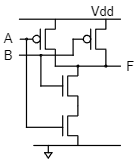
\includegraphics[width=0.35\linewidth]{Images/7}
	\caption{CMOS NAND-Gate}
	\label{fig:7}
\end{figure}
	
	\[
	F = \overline{A \cdot B}
	\]
	\newpage
	The truth table for a 2-input NAND gate is shown below:
	
	\begin{table}[H]
		\centering
			\caption{Truth Table for 2-Input CMOS NAND Gate}
		\begin{tabular}{|c|c|c|}
			\hline
			\textbf{A} & \textbf{B} & \textbf{F (NAND Output)} \\ \hline
			0          & 0          & 1                       \\ \hline
			0          & 1          & 1                       \\ \hline
			1          & 0          & 1                       \\ \hline
			1          & 1          & 0                       \\ \hline
		\end{tabular}
	
		\label{tab:nand_gate}
	\end{table}
	
	\subsection{2-Input CMOS AND Gate}
	The 2-input CMOS AND gate can be derived by using a 2-input NAND gate followed by a CMOS inverter. This configuration results in the output F being high only when both inputs A and B are high. The logic function of the 2-input CMOS AND gate is given as:
	
\begin{figure}[H]
	\centering
	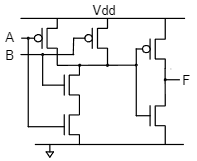
\includegraphics[width=0.45\linewidth]{Images/8}
	\caption{CMOS AND-Gate}
	\label{fig:8}
\end{figure}
	
	
	\[
	F = A \cdot B
	\]
	
	The truth table for a 2-input AND gate is shown below:
	
	\begin{table}[H]
		\centering
			\caption{Truth Table for 2-Input CMOS AND Gate}
		\begin{tabular}{|c|c|c|}
			\hline
			\textbf{A} & \textbf{B} & \textbf{F (AND Output)} \\ \hline
			0          & 0          & 0                       \\ \hline
			0          & 1          & 0                       \\ \hline
			1          & 0          & 0                       \\ \hline
			1          & 1          & 1                       \\ \hline
		\end{tabular}
	
		\label{tab:and_gate}
	\end{table}
	\newpage
	\subsection{1-Finger and 2-Finger MOS Fabrication}
	MOS transistors can be designed using different fabrication techniques to optimize the performance, area, and power consumption. \\
	In the context of semiconductor design, \textbf{"1 finger MOS"} refers to a single-gate Metal Oxide Semiconductor (MOS) transistor where the gate electrode is a single, continuous strip, while \textbf{"2 finger MOS"} means the gate is divided into two separate, parallel strips, essentially creating two smaller "fingers" of the gate, all sharing the same source and drain regions; the key difference is the number of gate fingers, which affects the transistor's electrical characteristics, particularly its current handling capability and parasitic capacitance.\\
	By dividing the gate into multiple fingers, the effective gate width increases, allowing for a higher current flow while maintaining a smaller overall transistor area.\\
	\begin{figure}[H]
		\centering
		\begin{subfigure}[t]{0.49\textwidth}
			\centering
			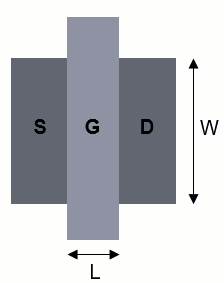
\includegraphics[width=.75\linewidth]{images/9.2}
			\caption{1 Finger MOS}
		\end{subfigure}
		\hfill
		\begin{subfigure}[t]{0.49\textwidth}
			\centering
			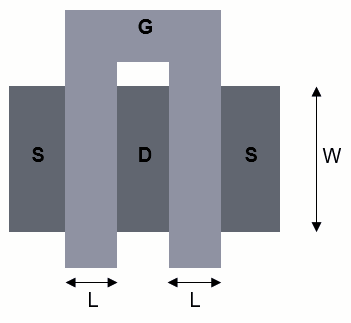
\includegraphics[width=1\linewidth]{images/10.3}
			\caption{2 Finger MOS}
		\end{subfigure}

	\caption{Multiple fingers layout (MOSFET transistor)}
	\label{fig:9}
\end{figure}
	\subsubsection{Advantages}
	\begin{enumerate}
\item 	\textbf{Improved RF performance:} Multi-finger design reduces gate resistance, leading to better high-frequency performance in RF circuits. 
\item 	\textbf{Lower parasitic capacitance:} Dividing the gate into smaller sections can decrease parasitic capacitance, improving circuit speed and power efficiency. 
\item \textbf{	Better matching:} When designing identical transistors with multiple fingers, the matching between them is often improved due to the similar layout and reduced variations.
	\end{enumerate}

	


	\newpage
	\section{Schematic Layout }
	\subsection{NAND GATE using 1 Finger MOS}
	\begin{figure}[H]
		\centering
		\includegraphics[width=1\linewidth]{"D:/DOWNLOAD 2024 V2/LATEX FILE/EEE_2214/EXP03_EEE2214/Images/4"}
		\caption{2 Input NAND-Gate using 1 Finger MOS}
		\label{fig:4}
	\end{figure}
	
	\subsection{AND Gate using 1 Finger MOS}
	
	\vspace{2cm}
	\begin{figure}[H]
		\centering
		\includegraphics[width=1\linewidth, height=0.6\textheight]{"D:/DOWNLOAD 2024 V2/LATEX FILE/EEE_2214/EXP03_EEE2214/Images/5"}
		\caption{2 Input AND-Gate using 1 Finger MOS and a CMOS}
		\label{fig:5}
	\end{figure}
	\subsection{NAND Gate using 2 Finger MOS}
		\vspace{1.5cm}
	\begin{figure}[H]
		\centering
		\includegraphics[width=0.5\linewidth]{"D:/DOWNLOAD 2024 V2/LATEX FILE/EEE_2214/EXP03_EEE2214/Images/1"}
		\caption{2 Input NAND-Gate using 2 Finger MOS }
		\label{fig:1}
	\end{figure}
	
	\newpage
	\subsection{AND Gate using 2 Finger MOS}
		\vspace{0.5cm}
	\begin{figure}[H]
		\centering
		\includegraphics[width=1\linewidth]{"D:/DOWNLOAD 2024 V2/LATEX FILE/EEE_2214/EXP03_EEE2214/Images/2"}
		\caption{2 Input AND-Gate using 2 Finger MOS and a CMOS }
		\label{fig:2}
	\end{figure}
	
	\section{Specification}
	\begin{table}[H]
		\centering
			\caption{MOSFET Dimensions for nMOS and pMOS Transistors}
		\label{tab:MOSFET_dimensions}
		\begin{tabular}{|c|c|c|c|c|}
			\hline
			\textbf{MOS} & \textbf{\begin{tabular}[c]{@{}c@{}}Width\\ ($\mu m$)\end{tabular}} & \textbf{\begin{tabular}[c]{@{}c@{}}Length\\ ($\mu m$)\end{tabular}} & \textbf{\begin{tabular}[c]{@{}c@{}}Width\\ ($\lambda$)\end{tabular}} & \textbf{\begin{tabular}[c]{@{}c@{}}Length\\ ($\lambda$)\end{tabular}} \\ \hline
			nMOS & 0.600 & 0.120 & 10 & 2 \\ \hline
			pMOS & 0.600 & 0.120 & 10 & 2 \\ \hline
		\end{tabular}
	
	\end{table}
	
		\begin{table}[H]
		\centering
			\caption{Parameters of Input Clock Signal for 1 Finger NAND-Gate and AND-Gate}
		% Sub-table (a)
		\begin{subtable}[t]{0.48\textwidth} % Adjusted width for each sub-table
			\centering
			\begin{tabular}{|c|c|c|}
				\hline
				\textbf{Parameter}          & \textbf{Value} & \textbf{Unit} \\ \hline
				High Level $(V)$            & 5.00           & $V$           \\ \hline
				Low Level $(V)$             & 0.00           & $V$           \\ \hline
				Time Low $(tl)$             & 0.225          & $ns$          \\ \hline
				Rise Time $(tr)$            & 0.002          & $ns$          \\ \hline
				Time High $(th)$            & 0.225          & $ns$          \\ \hline
				Fall Time $(tf)$            & 0.002          & $ns$          \\ \hline
			\end{tabular}
			\caption{Input clock signal of A} % Sub-table (a) caption
		\end{subtable}
		\hfil
		% Sub-table (b)
		\begin{subtable}[t]{0.48\textwidth} % Adjusted width for each sub-table
			\centering
			\begin{tabular}{|c|c|c|}
			\hline
			\textbf{Parameter}          & \textbf{Value} & \textbf{Unit} \\ \hline
			High Level $(V)$            & 5.00           & $V$           \\ \hline
			Low Level $(V)$             & 0.00           & $V$           \\ \hline
			Time Low $(tl)$             & 0.452         & $ns$          \\ \hline
			Rise Time $(tr)$            & 0.002          & $ns$          \\ \hline
			Time High $(th)$            & 0.452          & $ns$          \\ \hline
			Fall Time $(tf)$            & 0.002          & $ns$          \\ \hline
		\end{tabular}
			\caption{Input clock signal of B} % Sub-table (b) caption
		\end{subtable}
	\end{table}
	
	\begin{table}[H]
		\centering
		\caption{Parameters of Input Clock Signal for 2 Finger NAND-Gate and AND-Gate}
		% Sub-table (a)
		\begin{subtable}[t]{0.48\textwidth} % Adjusted width for each sub-table
			\centering
			\begin{tabular}{|c|c|c|}
				\hline
				\textbf{Parameter}          & \textbf{Value} & \textbf{Unit} \\ \hline
				High Level $(V)$            & 5.00           & $V$           \\ \hline
				Low Level $(V)$             & 0.00           & $V$           \\ \hline
				Time Low $(tl)$             & 0.452         & $ns$          \\ \hline
				Rise Time $(tr)$            & 0.002          & $ns$          \\ \hline
				Time High $(th)$            & 0.452          & $ns$          \\ \hline
				Fall Time $(tf)$            & 0.002          & $ns$          \\ \hline
			\end{tabular}
			\caption{Input clock signal of A} % Sub-table (a) caption
		\end{subtable}
		\hfil
		% Sub-table (b)
		\begin{subtable}[t]{0.48\textwidth} % Adjusted width for each sub-table
			\centering
			\begin{tabular}{|c|c|c|}
				\hline
				\textbf{Parameter}          & \textbf{Value} & \textbf{Unit} \\ \hline
				High Level $(V)$            & 5.00           & $V$           \\ \hline
				Low Level $(V)$             & 0.00           & $V$           \\ \hline
				Time Low $(tl)$             & 0.225          & $ns$          \\ \hline
				Rise Time $(tr)$            & 0.002          & $ns$          \\ \hline
				Time High $(th)$            & 0.225          & $ns$          \\ \hline
				Fall Time $(tf)$            & 0.002          & $ns$          \\ \hline
			\end{tabular}
			\caption{Input clock signal of B} % Sub-table (b) caption
		\end{subtable}
		
		
		
	\end{table}
	\begin{table}[H]
		\centering
			\caption{Parameters for Vdd+ and Vss- }
		\begin{tabular}{|c|c|c|}
			\hline
			\textbf{Parameter} & \textbf{Value} & \textbf{Unit} \\ \hline
			Vdd+               & 5.00           & $V $            \\ \hline
			Vss-               & 0.00           & $V$             \\ \hline
		\end{tabular}
		
	\end{table}

	\newpage
	\section{Output Waveshape }
	\subsection{NAND-Gate \& AND-Gate using 1 Finger MOS}
	\begin{figure}[H]
		\centering
		\includegraphics[width=1\linewidth]{"D:/DOWNLOAD 2024 V2/LATEX FILE/EEE_2214/EXP03_EEE2214/Images/1nand"}
		\caption{Output Waveshape of 2 Input NAND-Gate using 1 Finger MOS}
		\label{fig:1nand}
	\end{figure}
	\vspace{1.5cm}
	\begin{figure}[H]
		\centering
		\includegraphics[width=1\linewidth]{"D:/DOWNLOAD 2024 V2/LATEX FILE/EEE_2214/EXP03_EEE2214/Images/1and"}
		\caption{Output Waveshape of 2 Input NAND-Gate and AND-Gate using 1 Finger MOS }
		\label{fig:1and}
	\end{figure}
	
	\newpage
\subsection{NAND-Gate \& AND-Gate using 2 Finger MOS}
	
	\begin{figure}[H]
		\centering
		\includegraphics[width=1\linewidth]{"D:/DOWNLOAD 2024 V2/LATEX FILE/EEE_2214/EXP03_EEE2214/Images/2nand"}
		\caption{Output Waveshape of 2 Input NAND-Gate using 2 Finger MOS}
		\label{fig:2nand}
	\end{figure}
	\vspace{1.5cm}
	\begin{figure}[H]
		\centering
		\includegraphics[width=1\linewidth]{"D:/DOWNLOAD 2024 V2/LATEX FILE/EEE_2214/EXP03_EEE2214/Images/2and"}
		\caption{Output Waveshape of 2 Input NAND-Gate and AND-Gate using 2 Finger MOS }
		\label{fig:2and}
	\end{figure}
	\newpage
\section{Discussion}
The characteristics of 2-input CMOS NAND and AND gates were analyzed based on the input signals \(A\) and \(B\) and the corresponding output signal \(F\). It was observed that the output of the AND gate was the complement of the output of the NAND gate for all input combinations, indicating that they are logical inverses of each other. The truth tables verified that when the AND gate output is logic high, the NAND gate output is logic low, and vice versa.\\

During testing, the NAND gate exhibited some initial voltage flickering during state transitions, which was not observed in the AND gate. This behavior in the NAND gate was likely due to initial charge and discharge dynamics associated with its internal structure and switching characteristics. Despite the flickering, both gates followed the expected logical behavior as described in the truth table.

	
\end{document}